\documentclass[screen,citenumeric,long,10pt]{nrdoc}
%\documentclass[twoside,citenumeric,long,10pt]{nrdoc_060418}
\usepackage{citesort}     % Virker ikke...
\usepackage{multicol}
%\usepackage{subfigure}
\usepackage{fancyvrb}     % For crava model file
\usepackage{bm}           % For bold greek letters  --> /bm{theta}
%\usepackage{showlabels}
%\usepackage{floatflt}
%\usepackage{wrapfig}

% -------------------------------------------------
\title{CRAVA User Manual}
\subject{CRAVA User Manual}
\frontpagefigure{images/FFT_flowdiagram} % No file extension.
\keywords{CRAVA, seismic, inversion, geostatistical, Bayesian, AVO, FFT}
\author{P{\aa}l Dahle\and Bj{\o}rn Fjellvoll\and Ragnar Hauge\and Odd Kolbj{\o}rnsen\and Anne-Randi Syversveen}
\authorpdf{P{\aa}l Dahle, Bj{\o}rn Fjellvoll, Ragnar Hauge, Odd Kolbj{\o}rnsen and Anne-Randi Syversveen}
\aboutauthors{P{\aa}l Dahle is a Senior Research Scientist at NR,\\
              Bj{\o}rn Fjellvoll is a Senior Research Scientist at NR,\\
              Ragnar Hauge  is a Chief Research Scientist at NR,\\
              Odd Kolbj{\o}rnsen is a Chief Research Scientist at NR, and
              Anne-Randi Syversveen is a Senior Research Scientist at NR.}
\availability{Open to targets}
\project{n/a}
\projectnumber{n/a}
\reportnumber{SAND/04/2008}
\target{NR, StatiolHydro, Norsar}
\researchfield{Reservoir characterisation}
% ------------------------------------------------

\makeindex

\newcommand{\vect}[1]{\ensuremath{\mathbf{#1}}}
\newcommand{\bmu}{\bm\mu}
\newcommand{\bSigma}{\mbox{\large\ensuremath{\boldsymbol{\Sigma}}}}
%\newcommand{\vp}{\ensuremath{\alpha}\xspace}     % V_{p}
%\newcommand{\vs}{\ensuremath{\beta}\xspace}      % V_{s}
\newcommand{\vp}{\ensuremath{V_p}\xspace}      % V_{p}
\newcommand{\vs}{\ensuremath{V_s}\xspace}      % V_{s}
\newcommand{\avp}{a_{\alpha}}
\newcommand{\avs}{a_{\beta}(\vec{x},t,\theta)}
\newcommand{\arho}{a_\rho(\vec{x},t,\theta)}
\newcommand{\cml}{\nu_m}
\newcommand{\cel}{\nu_e}
\newcommand{\cmt}{\nu_m}
\newcommand{\cet}{\nu_e}
%\newcommand{\cmt}{r_{\!m}}
%\newcommand{\cet}{r_{\!e}}
\newcommand{\rms}   {\textsf{Irap RMS}\xspace}
\newcommand{\crava} {\textsf{CRAVA}\xspace}
\newcommand{\storm} {\textsf{Storm}\xspace}
\newcommand{\matlab}{\textsf{MATLAB}\xspace}
\newcommand{\perl}  {\textsf{Perl}\xspace}
\newcommand{\scriptref}[2]{\ifthenelse{\boolean{screen}}
  {\hyperref[#1]{#2}}{#2 (see \ref{#1})}}

\newcommand{\kw}[1]{\hyperref[#1]{\texttt{<#1>}}}
\newcommand{\rkw}[2]{\hyperref[#2]{\texttt{<#1>}}}

%\renewcommand\floatpagefraction{.80}

\addtolength{\abovecaptionskip}{-0.4em}

\begin{document}

\maketitle

\begin{abstract}
The CRAVA user manual
\end{abstract}

\tableofcontents
\clearemptydoublepage

\chapter{Bayesian inversion theory}
\label{sec:geostat-theory}
\index{Bayesian inversion}
\begin{multicols}{2}

\section{Introduction}
Seismic inversion has traditionally been treated as a deterministic
problem. However, there are several uncertain aspects: There is noise
in the seismic amplitude data, and the frequency resolution is
limited, so neither high nor low frequencies can be resolved from the
seismic data alone. Using a geostatistical approach to the problem of
seismic inversion, the uncertainty may be treated in a consistent and
robust way.

The \crava program uses the Bayesian linearised AVO
inversion method of Buland {\it et. al}~\cite{geo68ab2} to take
the uncertainty in seismic data into account. The seismic data are
described using multi-normal distributions, and modelled as the seismic
response of the earth model plus an error term. The earth model and
error term are modelled as multi-normal distributions in which spatial
coupling is imposed by correlation functions. Using a Bayesian
setting, prior models for the earth and error terms are set up based
on prior knowledge obtained from well logs, and the process of seismic
inversion is reduced to that of finding a posterior distribution for
the earth given the seismic data. The linearised relationship between
the model parameters and the AVO data, makes it possible to obtain the
posterior distribution analytically.

The posterior distribution for earth model parameters \vp
(pressure-wave velocity), \vs (shear-wave velocity), and $\rho$
(density), gives a laterally consistent seismic inversion. The lateral
correlation follows the stratigraphy of the inversion interval by
following the top and base of the inversion volume. As a consequence
of the spatial coupling, the solution in each location depends on the
solutions in all other locations. From the posterior distribution the
best estimate of the model parameters and a corresponding uncertainty
can be extracted. Moreover, since the distribution is normal, kriging
can be used to match the well data, and the posterior covariance can
be computed. This spreads full frequency information in an area around
the wells. Full frequency realizations can be generated by sampling
from the posterior distribution. A set of such realizations represents
the uncertainty of the inversion.

\section{AVO}
Amplitude versus offset (AVO) inversion can be used to extract
information about the elastic subsurface parameters from the angle
dependency in the reflectivity, see e.g.,
\cite{hamp90,lort93,pan94,bula96b}. In practice, and especially for
3-D surveys, linearised AVO inversion is attractive since it can be
performed with use of moderate computer resources. Prior to a
linearised AVO inversion, the seismic data must be processed to remove
nonlinear relations between the model parameters and the seismic
response. Important steps in the processing are the removal of the
moveout, multiples, and the effects of geometrical spreading and
absorption. The seismic data should be prestack migrated, such that
dip related effects are removed. After prestack migration, it is
reasonable to assume that each single bin-gather can be regarded as
the response of a local 1-D earth model. The benefits of prestack
migration before AVO analysis are discussed in
\cite{brow92,mosh96,bula2001d}. It is further assumed that wave mode
conversions, interbed multiples and  anisotropy effects can be
neglected after processing.  Finally, the prestack gathers must be
transformed from offsets to reflection angles.

\section{Geophysical model}

The seismic response of an isotropic, elastic medium is completely
described by the three material parameters $\{\vp(\vect{x},t),
\vs(\vect{x},t), \rho(\vect{x},t)\}$, where the vector $\vect{x}$
gives the lateral position (x,y), and $t$ is the vertical seismic
travel time.

The weak contrast approximation by Aki and Richards~\cite{aki80},
relates the seismic PP reflection coefficients $c(\vect{x},t,\theta)$
to the elastic medium, and is a linearisation of the Zoeppritz
equations (see Ref.\cite{aki80}). A continuous version of this
approximation is given by Stolt and Weglein~\cite{stolt85}:
%
\begin{equation}
\begin{split}
  c(\vect{x},t,\theta)
  & = a_{V\!p} (\theta) \frac{\partial}{\partial t}\ln\vp (\vect{x},t)\\
  & + a_{V\!s} (\vect{x},t,\theta) \frac{\partial}{\partial t}\ln\vs (\vect{x},t)\\
  & + a_\rho(\vect{x},t,\theta) \frac{\partial}{\partial t}\ln\rho(\vect{x},t),
\label{aki_c}
\end{split}
\end{equation}
%
where $\theta$ is the reflection angle, and
%
\begin{alignat}{2}
  &a_{V\!p} (\theta)            &&= \frac{1}{2}\left(1 + \tan^2\theta\right), \nonumber \\
  &a_{V\!s} (\vect{x},t,\theta) &&= -4 \frac{\vs^2(\vect{x},t)}
                                         {\vp^2(\vect{x},t)}\sin^2\theta, \label{a_coef}\\
  &a_\rho(\vect{x},t,\theta)    &&= \frac{1}{2}\left(1
                                   -4\frac{\vs^2(\vect{x},t)}{\vp^2(\vect{x},t)}
                                        \sin^2\theta\right).\nonumber
\end{alignat}
%
These equations are linearised by replacing the ratio
$\vs(\vect{x},t)/\vp(\vect{x},t)$ with a constant value
$\bar\vp/\bar\vs$ when computing $a_{V\!s}$ and $a_\rho$.

The seismic data are represented by the convolutional model
%
\begin{equation} \label{timeconv}
   d_{obs}(\vect{x},t,\theta)
    =\int w(\tau,\theta) \: c(\vect{x},t-\tau,\theta) \: d\tau + e(\vect{x},t,\theta),
\end{equation}
%
where $w$ is the wavelet, and $e$ is an angle and location dependent
error term. The wavelet can be angle dependent, but independent of the
lateral position $\vect{x}$. The wavelet is assumed to be stationary
within a limited target window.

The signal-to-noise ratio is defined as the ratio of the energy in the
two terms in expression~(\ref{timeconv}), that is,
\index{signal-to-noise ratio}
%
\begin{equation} \label{SNR}
   S/N =  \| w * c\|^2 / \| e\|^2,
\end{equation}
%
\noindent
where the operator * denotes the convolution.

\section{Statistical model}

The elastic parameters $\vp(\vect{x},t)$, $\vs(\vect{x},t)$, and
$\rho(\vect{x},t)$ are assumed to be log-normal random
fields. This means that the distribution $\vect{m}(\vect{x},t) =
\left[\ln\vp(\vect{x},t),\ln\vs(\vect{x},t),\ln\rho(\vect{x},t)\right]^T$
is multi-normal or multi-Gaussian, that is,
%
\begin{equation}
  \vect{m}(\vect{x},t) \sim
  \mathcal{N}\left(\bmu_m(\vect{x},t),\bSigma_m(\vect{x}_1,t_1;\vect{x}_2,t_2)\right),
\label{mdist}
\end{equation}
%
where $\bmu_m(\vect{x},t)$ are the expectations of
$\vect{m}(\vect{x},t)$ and $\bSigma_m(\vect{x}_1,t_1;\vect{x}_2,t_2)$
gives the covariance structure. We assume that the covariance function
is stationary and homogeneous (i.e., translationally invariant), and
can be factorised as
%
\begin{equation}
  \bSigma_m(\vect{x}_1,t_1;\vect{x}_2,t_2)
    = \bSigma_{0,m} \: \cml(\xi) \cmt(\tau), \label{sigma_m}
\end{equation}
% <
where $\cml(\xi)$ and $\cmt(\tau)$ are correlation functions
depending on the lateral and temporal distances
$\xi = \|\vect{x}_2 - \vect{x}_1\|$ and $\tau=|t_2-t_1|$,
respectively, and $\bSigma_{0,m}$ is a $3\times 3$ covariance matrix
having the variances of $\ln\vp$, $\ln\vs$ and $\ln\rho$  as diagonal
elements and their covariances off the diagonal. Any valid covariance
structures may be used.

If we let $\vect{m}$ and $\vect{d}_{obs}$ be discrete representations
of $\vect{m}(\vect{x},t)$ and $d_{obs}(\vect{x},t,\theta)$ in a time
interval, equation \eqref{timeconv} may be written in matrix
notation as
%
\begin{equation}
  \vect{d}_{obs} = \vect{G}\vect{m}^{\prime} + \vect{e}
\end{equation}
%
\noindent
where $\vect{G}$ is a matrix encompassing discrete representations of
the wavelet and the coefficients $a_{Vp}$, $a_{V\!s}$, and $a_\rho$, and
the matrix $\vect{m}^{\prime}$ is a time derivative of $\vect{m}$. The
error matrix $\vect{e}$ is a time discretization of the error vector
$\vect{e}(\vect{x},t) = [e(\vect{x},t,\theta_1),\ldots,$
$e(\vect{x},t,\theta_{n_{\theta}})]^T$ and is assumed to be zero-mean
coloured Gaussian noise, that is,
%
\begin{equation}
  \vect{e}(\vect{x},t)
    \sim \mathcal{N}_{n_\theta}\left(\vect{0},
               \bSigma_e(\vect{x}_1,t_1;\vect{x}_2,t_2)\right).
\label{edist}
\end{equation}
%
The covariance of the error vector is
%
\begin{equation}
  \bSigma_e(\vect{x}_1,t_1;\vect{x}_2,t_2)
    = \bSigma_{0,e} \: \cel(\xi) \cet(\tau), \label{sigma_e}
\end{equation}
%
where $\bSigma_{0,e}$ is an $n_{\theta}\times n_{\theta}$
covariance matrix containing the noise variances for the different
reflection angles on the diagonal, and the covariances between the
angles off the diagonal. Furthermore, $\cel(\xi)$ and $\cet(\tau)$
are lateral and temporal correlation functions, similar to those
given for $\vect{m}(\vect{x},t)$ in equation~\eqref{sigma_m}.

Since the relationship between the reflection coefficients and the
elastic parameters given in equation~\eqref{aki_c} is linear, and
the elastic parameters are assumed Gaussian distributed, the
reflection coefficients become Gaussian. Moreover, since the
convolution is a linear operation and we have assumed a Gaussian error
model, the seismic data given in equation~\eqref{timeconv} are also
Gaussian distributed.

For the time-discretized seismic data $\vect{d}_{obs}$, this gives us
the multi-normal distribution
%
\begin{equation}
  \vect{d}_{obs} \sim
    \mathcal{N}_{n_d}\left(\bmu_d,\bSigma_d\right),
\label{ddist}
\end{equation}
%
where
%
\begin{align}
  &\bmu_d = \vect{G}\bmu^{\prime}_{m},\\
  &\bSigma_d = \vect{G}\bSigma^{\prime\prime}_{m}\vect{G}^T + \bSigma_e.
\end{align}
%
where all vectors and matrices are time-discretized. The matrix
$\bSigma^{\prime\prime}_{m}$ is a doubly time-derivative of the
covariance matrix $\bSigma_m$.

This means that the simultaneous distribution for $\vect{m}$ and
$\vect{d}_{obs}$ is Gaussian, and that the distribution for $\vect{m}$
given $\vect{d}_{obs}$ can be obtained analytically using standard
theory for Gaussian distributions:
%
\begin{alignat}{2}
  &\bmu_{m|d_{obs}}    &&=\bmu_{m} +\bSigma_{d,m}^T \bSigma_{d}^{-1}
                           (\vect{d}_{obs}-\bmu_{d})     \label{mu_post} \\
  &\bSigma_{m|d_{obs}} &&=\bSigma_{m} - \bSigma_{d,m}^T
                           \bSigma_{d}^{-1}\bSigma_{d,m},\label{Sigma_post}
\end{alignat}
%
where $\bmu_{d}$ is the expected observation, that is, the
seismic response of $\bmu_m$, and $\bSigma_{d,m}$ is the
covariance matrix between logarithmic parameters and
observations. See Ref.~\cite{geo68ab1} for a detailed description on
how to compute these.

The computations given in equations~\eqref{mu_post}
and~\eqref{Sigma_post} involves the inverse of $\bSigma_{d}$. Given an
inversion volume with $n$ cells, this matrix has $n_\theta^2n^2$
elements, and for any reasonably sized volumes, inverting this matrix
is forbiddingly time consuming. However, the covariance function for a
homogeneously correlated spatial variable is diagonalised by a 3D
Fourier transform~\cite{christakos92}, and in this domain the inversion
problem can be solved independently for each frequency component. This
reduces the complexity of the computations dramatically, and the
calculation time becomes $\mathcal{O}(n\log n)$. This is illustrated
in Figure~\ref{fig:FFT-flowdiagram}. Details can be found in
Ref.~\cite{geo68ab2}
\index{FFT}

\chapter{Implementation}
\label{sec:implementation}
\index{CRAVA!implementation}


NBNB Ragnar: Skriv denne biten p� nytt.

\section{Using fft for inversion}
\section{Local wavelet and noise}
\section{Estimation of parameters}
\subsection{Estimating wavelet and noise}
\subsection{Estimating correlations}
\subsection{Estimating background model}

The \crava program gives an efficient implementation of the posterior
distribution given in equations \eqref{mu_post} and
\eqref{Sigma_post}, both in terms of computation and storage.

As prior information\index{prior model}, \crava estimates the
expectations $\bmu_m$, the correlation matrix $\bSigma_{0,m}$, and the
temporal correlation function $\cmt(\tau)$ directly from well
data. The lateral correlation functions $\cml(\xi)$ and $\cel(\xi)$
may be estimated from the seismic cubes, but unless the inversion

\begin{figure}[H]
  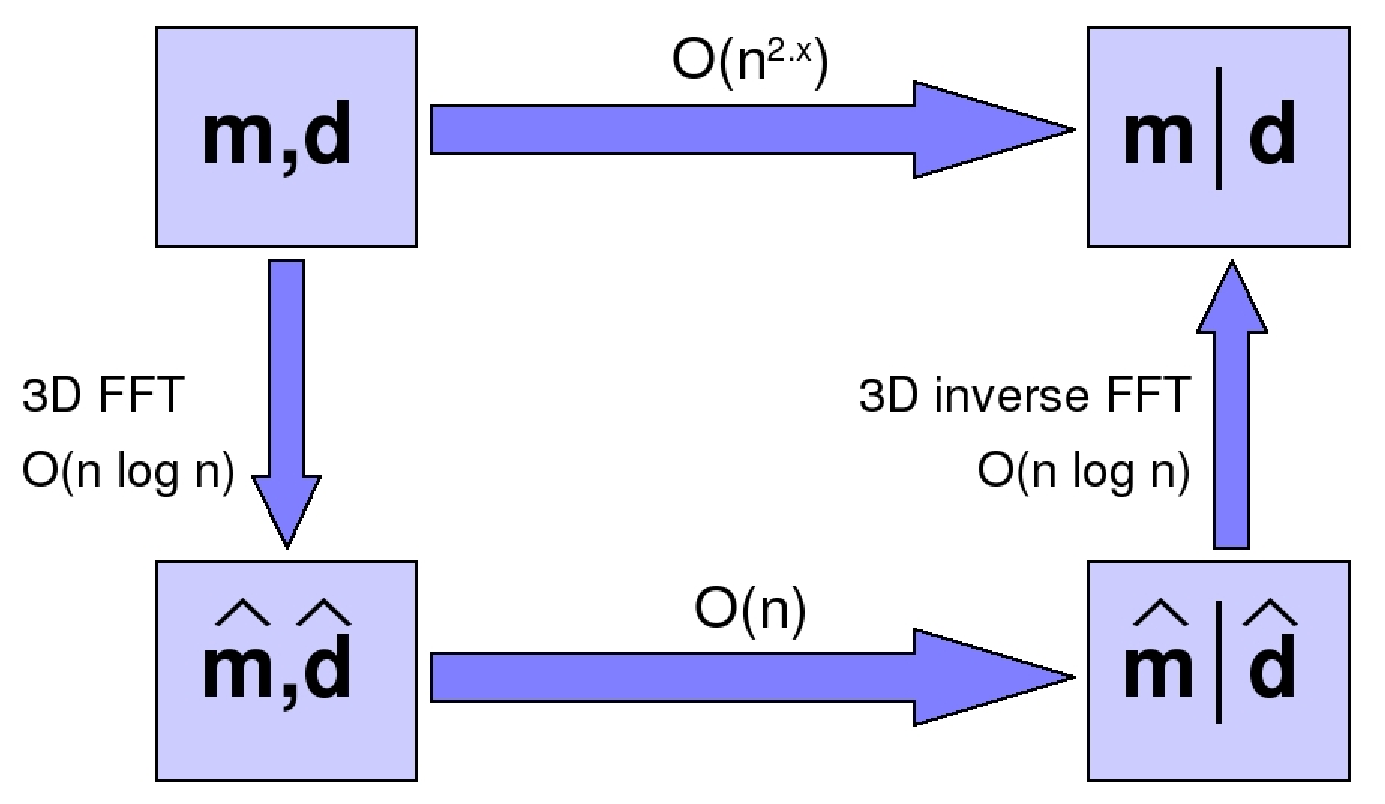
\includegraphics[width=.99\linewidth]{images/FFT_flowdiagram}
  \caption{The problem is transformed to the Fourier domain, solved
  in this domain, and back-transformed to time domain. This reduces
  the problem from a $\mathcal{O}(n^{2.x})$ to a $\mathcal{O}(n\log
  n)$ process.}
  \label{fig:FFT-flowdiagram}
\end{figure}

\noindent
interval is perfectly layered and the top and base surfaces follow
this layering exactly, the correlation ranges become
underestimated. As this may lead to numerical instabilities, a
parametric correlation function is typically used. In this case, the
same function is used for both correlations, and the correlation
function (type, ranges, and anisotropy angle) is given as input to the
program.

The error covariance matrix $\bSigma_{0,e}$ is also given as input
to the program. For an inversion system with two offsets $\theta_1$ and
$\theta_2$, the covariance matrix is
%
\begin{equation}
\bSigma_{0,e} =
\begin{bmatrix}
\sigma^2_{\theta_1}
& \sigma_{\theta_1}\sigma_{\theta_2}\nu_\theta(\phi)\\
\sigma_{\theta_1}\sigma_{\theta_2}\nu_\theta(\phi)
& \sigma^2_{\theta_1}\\
\end{bmatrix}
\end{equation}
%
\noindent
where $\sigma^2_{\theta_1}$ and $\sigma^2_{\theta_2}$ are the error
variances for offsets 1 and 2, respectively, and $\nu_\theta(\phi)$ is
an angular correlation function where $\phi=|\theta_2-\theta_1|$. The
variances and correlation function (type and range) are given as
\crava input.

The final part of the prior model, the error correlation function,
$\cet(\tau)$, consists of two parts. The first part gives the
correlation structure of the wavelet and is estimated by \crava, while
the other part is a white noise component and is given as program
input.

%\crava reads its input from a model file. In the model file the user
%specifies commands and parameters relevant for each command. There are
%commands available for specifying the seismic volumes, wavelets, and
%well data. The inversion region, the parts of the prior distribution
%not estimated by \crava, and the likelihood are also defined
%here. Finally, there are technical parameters that may be given, and
%commands for program output.

The model file used in the \crava run for the predicted parameters is
given in Appendix~\ref{sec:crava-model-file} for reference.
%
% The \newpage forces all text to appear in the left column only
% rather than a 50-50 split  between left and right columns...
%
\newpage
\chapter{User guide}
\label{sec:userguide}
\index{CRAVA!userguide}

In this chapter, we describe how to build a \crava model file. The model file mainly follows the XML-format, but we also use the character '\#' for commenting, meaning that the rest of the line after such a character is read as comment. All model files start with \kw{crava}, and end with \texttt{<\\crava>}.

\section{Basic inversion}
\label{sec:basicinv}
\index{inversion!basic}
A primary ability for \crava is to run simple first-pass inversions. In this section, we describe how to build a model file for a simple inversion.  
\subsection{Survey information}
\subsubsection{Seismic data}
\subsubsection{Wavelet}
\subsubsection{Noise}
\subsection{Inversion volume}
\subsubsection{Top and bottom surfaces}
\subsubsection{Lateral extent}
\subsubsection{Depth conversion}
\subsection{Background model and correlations}
\subsubsection{Background model}
\subsubsection{Correlations}
\subsection{Well data}
\subsection{Output}
\subsubsection{Grid output}
\subsubsection{Well output}
\subsection{Tasks}
%inversion, prediction/simulation
\section{Advanced inversion options}
\subsection{Non-stationary wavelet and noise}
\subsection{PS-seismic and reflection approximations}
\subsection{Well quality checks}
\subsection{Controlling lateral correlation}
\subsection{Depth conversion}
\subsection{Miscellaneous}
\section{Estimation}
\subsection{Wavelet estimation}
\subsection{Noise estimation}
\subsection{Background model estimation}
\section{Facies prediction}
\subsection{Prior probabilities}
\subsection{Relative versus absolute elastic parameters}
\section{Forward modelling}

\chapter{Reference manual}
\end{multicols}

%-----------------------------------------------------------------------------
%                                 APPENDIX
%-----------------------------------------------------------------------------

\appendix

%---------------------------------------------------

\chapter{Sample \crava model file}
\label{sec:crava-model-file}
\index{CRAVA!model file}

\vspace{-2em}

\begin{small}
\begin{Verbatim}[numbers=left]
PREFIX CRAVA_;

WELLS
HEADERS TWT DT RHOB DTS ;
/nr/project/sand/cravaruns/inputdata/logs/Well_1.rms
/nr/project/sand/cravaruns/inputdata/logs/Well_2.rms;

DEPTH
/nr/project/sand/cravaruns/inputdata/horizons/topsurface.storm
/nr/project/sand/cravaruns/inputdata/horizons/basesurface.storm
300;

BACKGROUND
/nr/project/sand/cravaruns/inputdata/background/BG_Vp.storm
/nr/project/sand/cravaruns/inputdata/background/BG_Vs.storm
/nr/project/sand/cravaruns/inputdata/background/BG_RHOB.storm;

SEISMIC
/nr/project/sand/cravaruns/inputdata/seismic/near.sgy                  15 .35
/nr/project/sand/cravaruns/inputdata/wavelets/wavelet_near_crava.txt             -0.80
/nr/project/sand/cravaruns/inputdata/seismic/far.sgy                   40 .39
/nr/project/sand/cravaruns/inputdata/wavelets/wavelet_far_crava.txt              -0.90;

FREQUENCYBAND   5 75;

ENERGYTRESHOLD  0.01;

SEGYOFFSET 2500;

PADDING 0.3 0.3 0.6;

LATERALCORRELATION  genexp 1 1500 500 0;
ANGULARCORRELATION  genexp 1 10;

WHITENOISE 0.1;

SEED 54667;

PREDICTION;

OUTPUT
AI RHO MURHO;
\end{Verbatim}
\end{small}

%---------------------------------------------------

\bibliography{references}

\end{document}
